Le \textit{system modeling} ou \textit{software modeling} correspond à la modélisation des briques logicielles qui feront le projet, il s’organise autour d’une réflexion des besoins, déjà évalués lors de la modélisation de données. 
Le projet sur la formation de l’Europe au XIIème siècle est confronté à un enjeu de durée s'étend sur 18 ans, période durant laquelle de nombreuses technologies apparaîtront et disparaîtront. Il s’agit d’une problématique commune à tous les projets envisagés sur le  long terme: quelles technologies utiliser?  Devons-nous tester, expérimenter avec les nouvelles technologies, les nouveaux logiciels et langages de programmation? \\
Il est nécessaire de rappeler que nous sommes à la genèse du projet sur le schisme alexandrin, les pistes évoquées ici sont hypothétiques. En revanche, l’objectif est aussi de tendre vers une réflexion plus vaste autour des attentes d’un projet long en humanités numériques. Pour aider dans cette réflexion, nous avons effectué des réunions avec les différents ingénieur.e.s du CCeH pour qu’ils nous introduisent aux différents projets en cours. Cela permettra d’analyser les forces et les faiblesses des technologies déjà utilisées au sein du CCeH.


    
    \chapter{Réunir les données}

Nous avons pu établir précédemment que les différents corpus documentaires sont pour la plupart déjà accessibles de manière dématérialisée, mais dispersés entre les différents projets d’humanités numériques. Le premier objectif, une fois le modèle de données établi, est donc de réfléchir à la manière dont nous souhaitons conserver ces données. Ainsi s’ouvre la réflexion à propos du choix de la base de données. 

    \section{Types de bases de données envisagées}

    \subsection{Le choix habituel en humanités numériques: base de données document}

Les données concernées sont pour une majorité d’entre elles au format XML. Le format XML est considéré comme un langage très pérenne\footnote{Pierazzo Elena, \textit{Textual Scholarship and Text Encoding}, in Schreibman Susan, Siemens Ray et Unsworth John, \textit{A new companion to Digital Humanities}, Wiley Blackwell, 2016, p307-321.}, et apparaît comme le choix le plus évident dans un projet d’humanités numériques comme celui-ci. Il est nécessaire dans ce cas d’utiliser une base de données de type document, qui permet de gérer des fichiers au format XML. Il y a deux grandes bases de données pour stocker nos données, chacunes ayant ses avantages et ses inconvénients:\\

\begin{itemize}
    \item eXist DB, qui est plutôt simple d’utilisation, permet de rapidement travailler sur les données et d’utiliser les frameworks XRX\footnote{Un framework correspond à un ensemble de logiciels et qui aide à utiliser du code mais qui impose un cadre précis dans le développement du frontend (partie visible pour les utilisateur.rice.s) et/ou le backend. En opposition, les librairies permettent également d’utiliser un ensemble de logiciels mais sans cadre imposé. Le framework XRX utilise Xforms (formulaire créé en XML), Rest et XQuery.}
    \item BaseX, qui permet de gérer une quantité importante de fichiers, et possibilité de connecter la base de données grâce à une API Rest.\\
    
\end{itemize}

\noindent Une base de données orientée document est un choix intéressant si le projet se concentre principalement sur la structure du document et à l’information qu’il contient. Elle permet de faire des recherches grâce aux balises, ce qui est spécifique aux bases de données XML. En revanche, plusieurs limites apparaissent en utilisant ce type de base de données:\\ 

\begin{itemize}
    \item Il faudra être très vigilant sur la normalisation des noms de personnes et de lieux afin d’éviter les doublons. Cela vaut également si l’on veut ajouter des noms grâce à un formulaire par exemple. Il est possible d’éviter les erreurs grâce aux attributs, mais cela signifie prendre du temps pour vérifier que les attributs soient entrés correctement
    \item Représenter des relations entre les personnes (liens familiaux par exemple) ou entre les personnes et les lieux devient complexe. C’est bien évidemment possible, mais c’est un travail fastidieux qui demande de créer des fichiers séparés pour l’ensemble des relations, qui apparaissent dans les attributs.
\end{itemize}
%En gros, si on souhaite voir les relations, il est nécessaire de créer et maintenir des index, dont les contraintes sont faites par des humains ==> plus de chances d'y avoir des erreurs
    
    \subsection{Les bases de données relationnelles}

Les bases de données relationnelles peuvent être une alternative aux bases de données document. Apparues dans les années 1980, les données y sont organisées en tables distinctes sans niveau de hiérarchie. Elles permettent de représenter les relations entre les différentes entités. Certaines bases de données relationnelles permettent de stocker des documents. On pense par exemple à PostgreSQL, qui offre un bon support du format JSON, avec de bonnes  performances à la clef. Pour un projet comme celui du CCeH, où le volume de données est assez faible comparé aux volumes que peuvent traiter les entreprises privées, stocker les documents dans une base relationnelle pour mieux tirer parti des autres avantages qu’offrent celles-ci est envisageable.\\ 
Un des avantages majeur à choisir une base de données relationnelle est de pouvoir exploiter des contraintes. Il s’agit de règles de maintien  de l’intégrité référentielle, une fois que vous définissez une règle, votre base de données vous empêchera de la violer en refusant les modifications qui contreviendraient à la règle. Cela vous permettra par exemple de définir les contraintes suivantes :\\
\begin{itemize}
    \item Chaque personne enregistrée en base de donnée ne doit l’être qu’une fois, il pourrait cependant avoir différents alias
    \item Les dates de naissances d’une personne doivent être définies de telle sorte que nul ne peut vivre plus de 130 ans
    \item La date d’édition d’une charte par un auteur doit être comprise entre son année de naissance et de décès
    \item Une personne ne peut pas voyager à plus de 60km/h. Formulé autrement, s’il est mention d’une même personne à deux points séparés d’une distance d et d’une durée t, alors d/t < 60.\\
    
\end{itemize}

\noindent Plus les contraintes sont précises et capturent la réalité du monde dans lequel s’inscrivent les données, plus vous serez capables d’identifier des incohérences dans vos jeux de données.\\
Autre avantage non négligeable des bases relationnelles : les relations elles-mêmes. Bien qu’il soit possible d’émuler un système relationnel dans une base documents, cela reste bien moins puissant que ce peut offrir les bases relationnelles et bien plus complexe à mettre en œuvre et maintenir.
Avec une extension pour la gestion des données géospatiales (PostGIS pour PostgreSQL par exemple), on peut imaginer la fonctionnalité suivante : requêter la base pour obtenir les tracés en GeoJSON des pays/régions administrés par des souverains soutenant Alexandre III chaque année de 1159 à 1181. Ces données permettraient de construire une carte intéractive des nations soutenant Alexandre III au cours de son exercice.

    
    \subsection{De nouvelles perspectives? Les bases de données graphe}

Une base de données orientée graphe est un modèle où la structure des données est représentée sous forme d’un graphe\footcite{angles_survey_2008}. Elle peut être utilisée lorsque l’on considère que les relations entre nos données sont au moins aussi importantes que les données elles-mêmes. Une base de données graphe permet de représenter le texte de la même manière que le XML le permet. En effet, un document XML a une structure conceptuelle d’arbre (XML Tree) et les arbres sont des graphes acycliques\footnote{Kosbie David, \textit{Data Structures: Trees and Graphs}}. 


\begin{figure}[H]
%centrer l'image
    \centering
    %commande qui permet de charger une image
    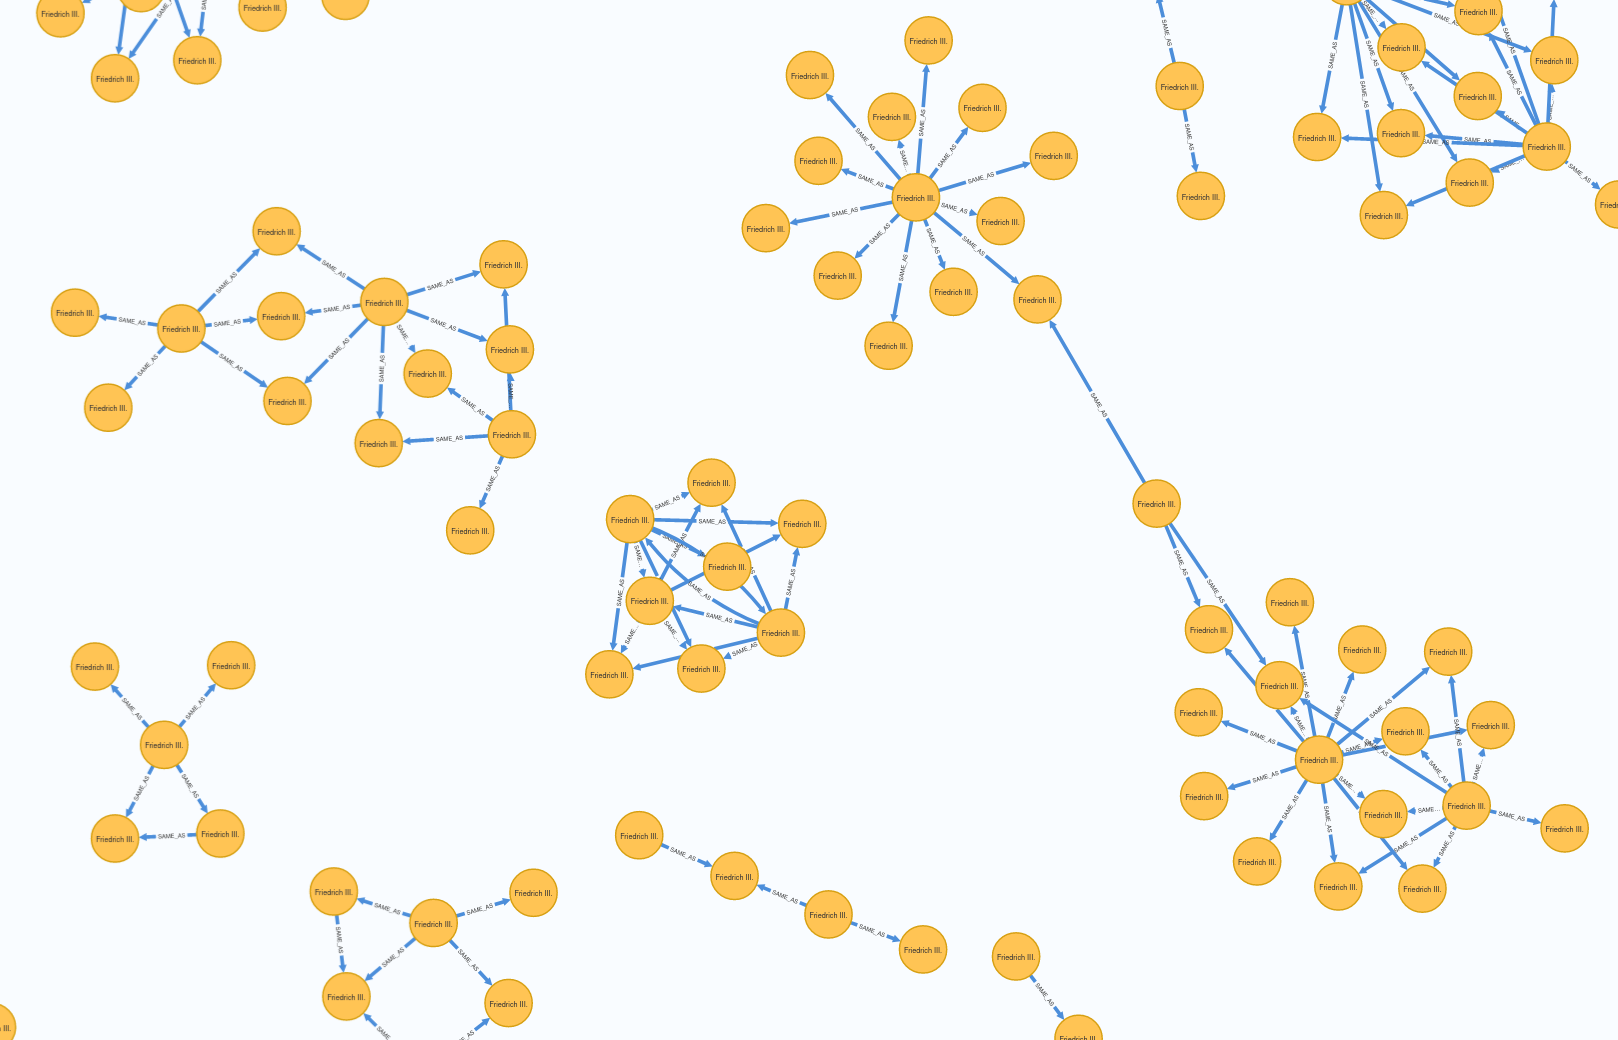
\includegraphics[width=14cm]{images/RI_graph.png}
    %légende
    \caption{Exemple de visualisation graphe avec des fichiers XML du RI Online}
    %label
    \label{fig:ExempleGraph}
\end{figure}

On peut voir par exemple ci-dessus un exemple avec des fichiers du RI Online \footnote{\url{https://kuczera.github.io/Graphentechnologien/23_\%C3\%9Cberlieferungsmodellierung.html}}. Les bases de données graphes sont parfois envisagées comme une alternative au XML, et les plus matures d’entre elles intègrent  de bonnes interfaces de visualisation de données. Les technologies graphe sont de plus en plus utilisées dans les humanités numériques, et particulièrement dans les centres de recherche allemands. On note par exemple les conférences  GrapHNR ou Graph Technologies in the Humanities\footnote{\url{ https://ceur-ws.org/Vol-3110/}}. Néanmoins, cela reste une technologie de niche: le site \url{datanyze.com} estime la part de marché de Neo4j (la base de données graphe la plus populaire) à 0.46\%. Pour un projet aussi long que celui du schisme alexandrin, le choix d’une base de données graphe ne serait sans doute pas le plus sûr; mais puisque celui-ci s’étend sur 18 ans, des expérimentations avec ce type de base de données ne sont pas à exclure.



    \section{Une base de données unique?}

Cette question peut paraître étonnante. En effet, dans beaucoup de projets comme celui-ci, il est courant d’utiliser une seule base de données, mais, en termes de durabilité et d’objectifs du projet, il faut questionner l’usage de différents types de bases pour répondre aux différents enjeux introduits par nos données. 


    \subsection{Avantages}

Il paraît beaucoup plus intuitif de stocker nos données au sein d'une même base. C’est humainement plus facile, car il n’y a qu’un seul langage de base de données à connaître, une seule connexion entre notre application et la base à gérer et enfin une seule base à maintenir  En effet, si on multiplie les moyens de stockage, on multiplie alors aussi les opérations de maintenance, les vulnérabilités potentielles, l’effort requis pour répliquer le projet, les sauvegardes et les compétences nécessaires à la compréhension du projet.\\ 
Par ailleurs, l’ajout d’une nouvelle base de données implique la gestion de la dépendance entre les données des deux bases. À l’instar d’une base de données relationnelle qui garantit l’intégrité référentielle entre les données de différentes tables, il nous faudra gérer l’interopérabilité des données de nos deux bases.\\
Néanmoins, s’astreindre à n’utiliser qu’une seule base de données - et donc une seule manière de représenter nos données - a aussi des inconvénients.
    
    \subsection{Inconvénients}

Si les données revêtent plusieurs formes, comme c’est le cas pour le projet du schisme Alexandrin, avoir une seule base de données impose plusieurs contraintes en termes d’exploitation des données. Par exemple, si le choix se porte sur une base de données XML, la partie relationnelle se révélera complexe à gérer. Au contraire, utiliser une base de données relationnelle en plus de celle document permettrait de plus facilement s’occuper des relations.\\ 
Dans le secteur privé, il est très courant de voir des projets utiliser plus d’une base de données. Chaque base répond à un besoin bien spécifique, qui fait qu’elle sera favorisée par rapport à une autre. Par exemple, s’il est nécessaire de mettre en place un cache pour accélérer l’application, il ne sera pas rare d’ajouter une base Redis au projet. Si nous souhaitons ajouter une fonctionnalité de recherche avancée à l’application, on peut alors utiliser ElasticSearch. Avoir plusieurs bases de données pour un seul projet est une pratique plutôt commune.\\


	Au final, réunir ses données dans une ou plusieurs bases de données, dans base de données relationnelles ou document, etc… est une décision à prendre en fonction de la manière dont on veut utiliser les données.
